\documentclass[a4paper]{jpconf}
\usepackage{graphicx}
\usepackage{color}
\usepackage{array}
\usepackage{enumerate}

\begin{document}
\title{WLCG and IPv6 - the HEPiX IPv6 working group}

\author{K. Chadwick$^1$, G. Chen$^2$, J. Chudoba$^3$, P. Clarke$^4$, M. Elias$^3$,
        A. Elwell$^5$, S. Fayer$^6$, Q. Fazhi$^2$, T. Finnern$^7$, L. Goossens$^5$,
        C. Grigoras$^5$, B. Hoeft$^8$, D. Kelsey $^9$, T. Kouba$^3$, 
        F. Lopez Mu\~noz$^{10}$, E. Martelli$^5$, M. Mitchell$^{11}$, A. Nairz$^5$, 
        K. Ohrenberg$^7$, A. Pfeiffer$^5$, F. Prelz$^{12}$, D. Rand$^6$, 
        M. Reale$^{13}$, S. Rozsa$^{14}$, R. Voicu$^{14}$, T. Wildish$^{15}$}

\address{$^1$ Fermi National Accelerator Laboratory, Batavia, Il 60510, U.S.A.}
\address{$^2$ Institute of High Energy Physics, 19B YuquanLu, Shijingshan District, 100049 Beijing, China} 
\address{$^3$ Institute of Physics, Academy of Sciences of the Czech Republic Na Slovance 2 182 21 Prague 8, Czech Republic}
\address{$^4$ The University of Edinburgh, Mayfield Road, Edinburgh EH9 3JZ, United Kingdom}
\address{$^5$ CERN, CH-1211 Gen\`eve 23, Switzerland}
\address{$^6$ Imperial College London, South Kensington Campus, London SW7 2AZ, United Kingdom}
\address{$^7$ Deutsches Elektronen-Synchrotron, Notkestra\ss e 85, D-22607 Hamburg, Germany}
\address{$^8$ Karlsruher Institut f\"ur Technologie, Hermann-von-Helmholtz-Platz 1, D-76344 Eggenstein-Leopoldshafen, Germany}
\address{$^9$ STFC Rutherford Appleton Laboratory, Harwell Oxford, Didcot, Oxfordshire OX11 0QX, United Kingdom}
\address{$^{10}$ Port d'Informaci\'o Cient\'ifica, Campus UAB, Edifici D, E-08193 Bellaterra, Spain}
\address{$^{11}$ University of Glasgow, Kelvin Building, University Avenue, Glasgow, G12 8QQ, United Kingdom}
\address{$^{12}$ INFN, Sezione di Milano, via G. Celoria 16, I-20133 Milano, Italy}
\address{$^{13}$ Consortium GARR, Via dei Tizii 6, I-00185 Roma, Italy}
\address{$^{14}$ California Institute of Technology, Pasadena, Ca 91125, U.S.A. }
\address{$^{15}$ Princeton University, Jadwin Hall, Princeton, NJ 08544, U.S.A.}

\ead{ipv6@hepix.org}

\begin{abstract}
The HEPiX ({\tt http://www.hepix.org}) IPv6 Working Group has 
been investigating the many issues which feed into the decision on the 
timetable for the use of IPv6 networking protocols in HEP Computing, in 
particular in WLCG. RIPE NCC, the European Regional Internet Registry, ran 
out of IPv4 addresses in September 2012. The North and South America RIRs 
are expected to run out in 2014. In recent months it has become more clear 
that some WLCG sites, including CERN, are running short of IPv4 address space, 
now without the possibility of applying for more. This has increased the 
urgency for the switch-on of dual-stack IPv4/IPv6 on all outward facing WLCG 
services to allow for the eventual support of IPv6-only clients. The 
activities of the group include the analysis and testing of the readiness 
for IPv6 and the performance of many required components, including the 
applications, middleware, management and monitoring tools essential for 
HEP computing. Many WLCG Tier 1 and Tier 2 sites are participants in the 
group's distributed IPv6 testbed and the major LHC experiment collaborations 
are fully engaged in the testing. We have worked closely with similar 
activities elsewhere, such as EGI and EMI. We are constructing a group 
web/wiki which will contain useful information for sites on the IPv6 
readiness of the various software components. This includes advice on 
IPv6 configuration and deployment issues for sites 
({\tt http://hepix-ipv6.web.cern.ch/knowledge-base}). \\
This paper will describe the work done by the HEPiX IPv6 working group 
since CHEP2012. This will include detailed reports on the testing of 
various WLCG services on IPv6 including data management, data transfer, 
workload management and system/network monitoring. It will also present 
the up to date list of those applications and services which function 
correctly in a dual-stack environment together with those that still 
have open issues. The plan for more testing on the production infrastructure 
with a dual-stack IPv4/IPv6 setup and the work required before the support 
of IPv6-only clients is realised will be described.
\end{abstract}

\section{Introduction}
%section 1

The HEPiX IPv6 Working Group \cite{ipv6wg} has been investigating the many issues involved in the deployment and use of
IPv6 in HEP in general and more specifically in WLCG. The group's paper at CHEP2016 \cite{ipv6chep2016}
presented the status then of the work to allow sites to deploy IPv6-only CPU resources. Driven by the
requirements of the LHC experiments, the WLCG Management Board, in September 2016, had approved our plan
that all WLCG Tier-2 storage services should aim to support dual-stack IPv6/IPv4 by the end of 2018. Since then the
group has worked with others to encourage, support and monitor that transition and to identify and help
solve any technical issues as they arise.

%This paper is organised as follows.  Section 2 presents the current status of the transition for the Tier0/Tier1s, the Tier2s and the Experiment Services.
%Section 3 presents an update on service availability and network monitoring and also reports on the fraction of FTS data transfers currently taking place over IPv6.
%Finally section 4 contains future plans and conclusions. 

 


\section{IPv6: the general problem}
blah blah


\section{The HEPiX IPv6 working group}
blah blah


\section{The IPv6 testbed}
The impact of IPv6 is not limited to the transport layer 
but introduces the need for choice and preference in name-to-address 
resolution, implies multi-homing of all network endpoints (possibly on 
multiple protocol versions) and requires opaque handling of address 
information. This broadens the scope of code changes needed to add
IPv6 support to existing code and adds to the complexity of testing:
continued operation on IPv4 on dual-stack hosts, then preference of IPv6 and 
options to control it for all network bindings and connections
need to be verified with adequate code coverage.
\par
At opposite ends of the spectrum of practical testing options are
testing of individual, isolated components and services and the analysis of 
integrated services on dual-stack nodes. Both approaches are incomplete:
\begin{itemize}
\item[-] testing of isolated components misses the interaction with other
services at the OS level and usually requires services to be configured
differently than for production;
\item[-] testing of production-ready, integrated nodes may just be 
accidentally focusing on normal operation and bring insufficient 
code and functionality coverage.
\end{itemize}
This calls for a complementary approach,
where individual services are deployed and tested within the scale of
available dedicated resources and, once sufficient confidence and knowledge
of their level and mode of IPv6 support is built, are watched in the context
of a production node with dual-stack network and dual IPv4/IPv6 public address
resolution.
\par
Desirable characteristics of a dedicated testbed for single-service testing are:
\begin{itemize}
\item Geographical spread covering all ranges of realistic network latencies
and as many network providers as possible.
\item Uniform authentication/authorization scheme to factor AA issues out.
\item Uniform OS installation, to factor out any issue with the custom 
configuration needed to test isolated services and for easier
deployment of new services.
\end{itemize}
The current list of active testbed nodes can be found at the following URL:\\
{\tt http://hepix-ipv6.web.cern.ch/content/testbed}\\
While we have at the time of writing a reasonable
9-site/6-NREN coverage of Europe, the only non-european site in the testbed
is IHEP at Beijing. More testbed sites are both needed and welcome to join 
to achieve a better match of our stated testbed goals.
\par
As for OS distributions, testbed nodes are mostly installed with 
Scientific Linux (CERN) version 5,
to replicate production conditions at LCG Tier-X centres. A few testbed nodes
have RHEL 6 derivatives installed: this allowed us to discover 
(and document in our knowledge base, {\tt http://hepix-ipv6.web.cern.ch/knowledge-base})
that, rather unexpectedly, {\tt libc} on RH6 causes unspecified 
protocol sockets to be bound on IPv4 only, instead of dual-stack 
as it used to be.
\par
To achieve the simplest possible authentication scheme, a custom Globus
Security Infrastructure (GSI)
plug-in maps all members of our test VO ({\tt ipv6.hepix.org}) to one
local account, logging any access. 
\par
The first service we deployed for standalone testing through testbed was
GSIFTP. This was not only because of GSIFTP's basic role in WLCG data
transfer, but also because the FTP protocol (the GSI extensions don't 
affect but also suffer from this issue) is a paradigmatic example of 
how non-trivial IPv6 support can be. The original FTP specifications 
(RFC765/RFC959) used the quad-byte notation for IP addresses 
{\em in the syntax of the FTP protocol commands} {\tt PORT} and {\tt PASV}.
This required the introduction, with RFC 2428 (September 1998) of
``extended'' versions of the same commands, supporting different address
families, and IPv6 in particular. We found on our testbed that support for 
the 'extended' command forms (and thus {\em implicitely} for IPv6)
is missing from certain FTP client implementations. Retrofitting the
clients with these commands is definitely more than a simple change in
the transport layer and serves as an example of how ramified the
introduction of 'IPv6 support' can be.
\par
Building on this mesh of GSIFTP servers, both continuous direct point-to-point 
file transfer tests and tests of the File Transfer Service 
(FTS), were successfully carried on. SRM endpoints
were also added, as described in detail in the next section.


\section{IPv6 testing and results}
\subsection{Testing testing...}
This is where the testing results go

some numbers for now: Transfers running since March, some 2.6 million transfers, 86.8 percent success
rate, over 2 PB of data so far. Approx. 7 percent of the rate CMS achieves globally.

The mesh...

\begin{figure}[htp]
\centering
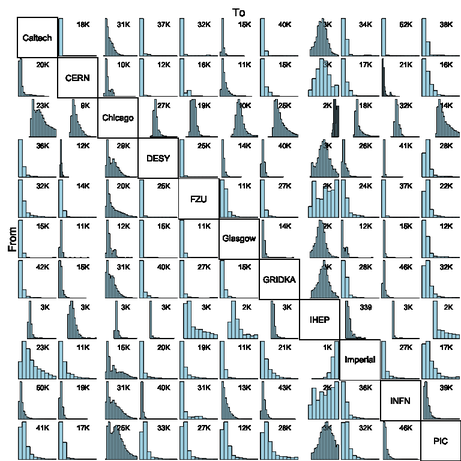
\includegraphics{full-mesh}
\caption{Transfer performance for the IPv6 testbed continuous transfers. A 1 GB file is transferred between each pair of sites, then deleted, then transferred again, continuously. The plots show the distribution of transfer duration times per site pair. The source site is named in the row, the destination site is named in the column. So the top-right plot shows transfers from Caltech to PIC, the bottom-left shows transfers fromPIC to Caltech. The x-axis is in seconds, from 0 to 500 for each plot. The number inset in each plot shows the approximate number of transfers between that site pair in that direction.}\label{fig:full-mesh}
\end{figure}



\section{Software and tools survey}
blah blah


\section{Collaboration with other groups}
blah blah


\section{Outlook and future plans}
blah blah


\section{Conclusions}
blah blah


\par
\begin{thebibliography}{}
%
% and use \bibitem to create references.
%
% Format for Journal Reference
%Journal Author, Journal \textbf{Volume}, page numbers (year)
% Format for books
%\bibitem{RefB}
%Book Author, \textit{Book title} (Publisher, place, year) page numbers
% etc


%section 1 references
%\bibitem{ipv6wg} The HEPiX IPv6 Working Group, http://hepix-ipv6.web.cern.ch
\bibitem{ipv6wg}
S. Campana et al, J. Phys. Conf. Ser. {\bf513}, 062026 (2014)



%\bibitem{ipv6chep2016} 
% M. Babik et al, J. Phys. Conf. Ser. {\bf898}, 082033 (2017)
\bibitem{ipv6chep2018} 
M. Babik et al, J. Phys. Conf. Ser. {\bf214}, 08010 (2019)

\bibitem{eos} A. J. Peters et al, J. Phys. Conf. Ser. {\bf664}, 042042 (2015)


%section 2 references

\bibitem{rfc} 
All Internet Engineering Task Force Requests For Comments (RFC) documents are available
from URLs such as https://www.ietf.org/rfc/rfcNNNN.txt where NNNN is the RFC number, for example {\tt https://www.ietf.org/rfc/rfc2460.txt}



%section 2 intro para

\bibitem{ipv6chep2015} 
J. Bernier et al, J. Phys. Conf. Ser. {\bf664}, 052018 (2015)

%section 2.1 Tier 0/1
\bibitem{fts3}
A.~A. Ayllon et al, 
%M~Salichos, M~K Simon, and O~Keeble.
%\newblock Fts3: New data movement service for wlcg.
J. Phys. Conf. Ser. {\bf 513}, 032081 (2014)

%section 2.2 Tier 2

%section 2.3 LHCOPN
\bibitem{opnone}
E. Martelli et al, J. Phys. Conf. Ser. {\bf 664}, 052025 (2015)

%section 2.4 Data transfers



%section 2 Experiments
%\bibitem{alien} 
%S. Bagnasco et al, J. Phys. Conf. Ser. {\bf119(6)}, 062012 (2008)

%\bibitem{xrootd}
%L. Bauerdick et al, J. Phys. Conf. Ser. {\bf 396} 042009 (2012)

%\bibitem{jalien}
%A. Grigora et al, J. Phys. Conf. Ser. {\bf523}, 012010 (2014)

%\bibitem{glideinwms} 
%http://iopscience.iop.org/article/10.1088/1742-6596/119/6/062044
%I. Sfiligoi, J. Phys. Conf. Ser. {\bf119(6)}, 062044 (2008)

%\bibitem{htcondor}
%D. Thain et al, Concurrency - Practice and Experience, {\bf 7(2-4)}, 323 (2005)

%\bibitem{dirac} A. Tsaregorodtsev et al, J. Phys. Conf. Ser. {\bf513}, 032096 (2014)

%LHCb : LHCb collaboration, A. A. Alves Jr. et al., The LHCb detector at the LHC, JINST 3 (2008) S08005

%section 3 references

%section 3.1
\bibitem{ipv6trans}
M. Nikkhah and R. Gu\'erin, 
IEEE/ACM Transactions on Networking, {\bf 24(4)}, 2291 (2016)

\bibitem{jool}
https://www.jool.mx

%section 3.2

\bibitem{RefLHCOPNEv4v6}
LHCOPN and LHCONE traffic flows on the CERN border routers, 
https://twiki.cern.ch/twiki/bin/view/LHCOPN/LHCOPNEv4v6Traffic


%section 3.3
\bibitem{frontier}
http://frontier.cern.ch/

%\bibitem{sam}
%A. Aimar et al, J. Phys. Conf. Ser. {\bf 898(9)}, 092033 (2017)
%A~Aguado Corman, P~Andrade, S~Belov, J~Delgado Fernandez, B~Garrido Bear, M~Georgiou, E~Karavakis, L~Magnoni, R~Rama Ballesteros, H~Riahi, J~Rodriguez Martinez, P~Saiz, and D~Zolnai.
%\newblock Unified monitoring architecture for it and grid services.


%\bibitem{etf}
%Marian Babik, CERN,
%\newblock Experiments {Test} {Framework} ({ETF}).
%http://etf.cern.ch/docs/latest/

%\bibitem{perfsonar} 
%A. Hanemann et al, 
%Jeff~W. Boote, Eric~L. Boyd, J{\'e}r{\^o}me Durand, Loukik
 %Kudarimoti, Roman {\L}apacz, D.~Martin Swany, Szymon Trocha, and Jason Zurawski.
%\newblock Perfsonar: A service oriented architecture for multi-domain network monitoring.
%\newblock In Boualem Benatallah, Fabio Casati, and Paolo Traverso, editors,
  %{\em Service-Oriented Computing - ICSOC 2005}, pages 241--254, Berlin, Heidelberg, 2005. Springer Berlin Heidelberg.

%\bibitem{wlcg-NTWG}
%S.~McKee et al, J. Phys. Conf. Ser. {\bf 664(5)} 052003 (2015)
%S.~Campana, A.~Di Girolamo, T.~Wildish, J.~Closier, S.~Roiser, C.~Grigoras, I.~Vukotic, M.~Salichos, Kaushik De, V.~Garonne, J.A.D. Cruz, A.~Forti, C.J. Walker, D.~Rand, A.~de~Salvo, E.~Mazzoni, I.~Gable, F.~Chollet, L.~Caillat, F.~Schaer, Hsin-Yen Chen, U.~Tigerstedt, G.~Duckeck, B.~Hoeft, A.~Petzold, F.~Lopez, J.~Flix, S.~Stancu, J.~Shade, M.~O'Connor, V.~Kotlyar, and J.~Zurawski.
%\newblock Integrating network and transfer metrics to optimize transfer efficiency and experiment workflows.


%\bibitem{psmad}  
%perfSONAR Consortium,
%\newblock {perfSONAR} {Monitoring and Debugging Dashboard (MADDASH)}.
%http://psmad.grid.iu.edu/toolkit/
%http://psmad.grid.iu.edu/maddash-webui/
%index.cgi?dashboard=OPN%20Mesh%20Config

%\bibitem{grafana-ipv6}
%CERN monitoring team,
%\newblock {CERN} {MONIT} {Grafana} {Dashboard}.
%https://monit-grafana.cern.ch/





%\bibitem{RefLHCOPNEv4v6}
%LHCOPN and LHCONE traffic flows on the CERN border routers, 
%https://twiki.cern.ch/twiki/bin/view/LHCOPN/LHCOPNEv4v6Traffic


%\bibitem{grafana-FTS}
%CERN~{MONIT} team.
%\newblock {CERN} {MONIT} {Grafana} {FTS} {Dashboard}.
 
%\bibitem{grafana-WLCG-Transfers}
%CERN~{MONIT} team.
%\newblock {CERN} {MONIT} {Grafana} {WLCG} {Transfers} {Dashboard}.


%\bibitem{xrootd-ipv6}
%SLAC~{XRootD} team.
%\newblock {XRootD System Monitoring Reference}.


%\bibitem{sam} A. Aimar et al, J. Phys. Conf. Ser. {\bf 898}, 092033 (2017)
%A.A. Corman, P. Andrade, S. Belov, J.D. Fernandez, B.G. Bear, M. Georgiou,E. Karavakis, L. Magnoni, R.R. Ballesteros et al., Unified Monitoring Architecture for IT and Grid Services


%\bibitem{etf} M. Babik,Experiments Test Framework (ETF), https://etf.cern.ch/docs

%\bibitem{perfsonar} A.  Hanemann et al,  
%J.W.  Boote,  E.L.  Boyd,  J.  Durand,  L.  Kudarimoti,  R.  Łapacz,  D.M.Swany, S. Trocha, J. Zurawski, PerfSONAR: A Service Oriented Architecture for Multi-domain Network Monitoring, inService-Oriented Computing  ICSOC 2005, edited by B. Benatallah et al (Springer Berlin Heidelberg, Berlin, Heidelberg,2005), pp. 241-254, ISBN 978-3-540-32294-8

%\bibitem{wlcg-NTWG}  S. McKee, M. Babik, S. Campana, A.D. Girolamo, T. Wildish, J. Closier, S. Roiser,C. Grigoras, I. Vukotic, M. Salichos et al., Integrating network and transfer metrics to optimize transfer efficiency and experiment workflows, Journal of Physics:  Conference Series664,052003 (2015)

%\bibitem{psmad} perfSONAR Consortium,perfSONAR Monitoring and Debugging Dashboard (MAD-DASH),http://psmad.opensciencegrid.org/maddash-webui/index.cgi

%\bibitem{grafana-ipv6} CERN  MONIT  Grafana  Dashboard,http://monit-grafana-open.cern.ch/d/000000809/perfsonar-ipv6



%section 4 references


\end{thebibliography}



\end{document}

